\section{Benchmark NIST-4 "Peak"}
\label{sec:bench-4}

The solution of this problem exhibits an exponential peak in the interior of the domain.
The equation solved in this benchmark problem is the Poisson's equation.

\begin{equation} \label{poisson-peak}
-\Delta u = f 
\end{equation}

in the domain $\Omega = (0, 1)^2$, equipped with Dirichlet
boundary conditions given by the exact solution.
The exact solution is

\begin{equation}\label{exact-nist-4}
u(x,y) = e^{-\alpha ((x - x_{loc})^{2} + (y - y_{loc})^{2})} 
\end{equation}

where $(x_{loc}, y_{loc})$ is the location of the peak,
and $\alpha$ determines the strength of the peak.
The right-hand side $f$ is calculated by inserting (\ref{exact-nist-4}) into (\ref{poisson-peak}).
The solution of NIST-4 with $\alpha = 1000$,
$(x_{loc}, y_{loc}) = (0.5, 0.5)$ is shown in Fig. \ref{fig:sln-nist04}.

\begin{figure}[!ht]
\centering
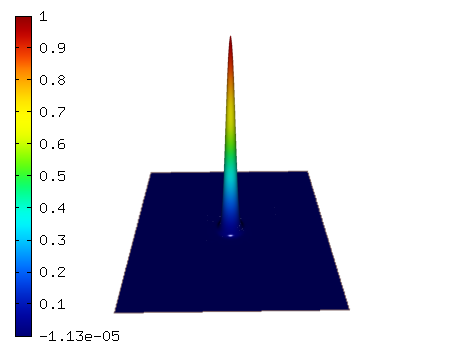
\includegraphics[height=5cm]{nist/nist-4/solution.png}
\caption{The solution to NIST-4 benchmark problem.}
\label{fig:sln-nist04}
\end{figure}

The goal of the benchmark is to reach a relative error below
$10^{-2}$~\% in the $H^1$-norm with as few DOFs as possible.
We begin with adaptive $hp$-FEM,
the initial mesh is shown in Fig. \ref{fig:nist-4-hp-aniso} (left).
After 12 adaptivity steps, the resulting mesh with 1561 DOF is shown
in Fig. \ref{fig:nist-4-hp-aniso} (right).

\begin{figure}[!ht]
\centering
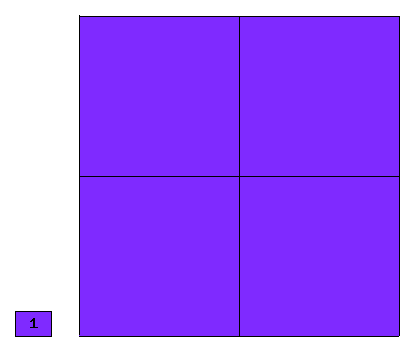
\includegraphics[height=5cm]{nist/nist-4/mesh_hp_aniso_init.png}\ \
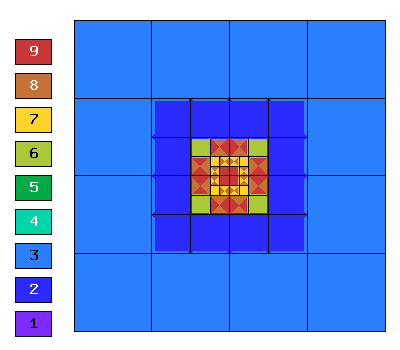
\includegraphics[height=5cm]{nist/nist-4/mesh_hp_aniso.png}
\caption{Initial mesh (left) and final mesh (right) for $hp$-FEM with anisotropic refinements.}
\label{fig:nist-4-hp-aniso}
\end{figure}

The final relative error estimate in $H^1$-norm was 7.02865e-03 \%,
and it was identical to the exact error in all printed digits.
We also solved this benchmark with adaptive $h$-FEM
with linear (left) and quadratic (right)
elements, with anisotropic refinements enabled.
Final meshes for the $h$-FEM computations are shown
in Fig. \ref{fig:nist-4-h-aniso}.

\begin{figure}[!ht]
\centering
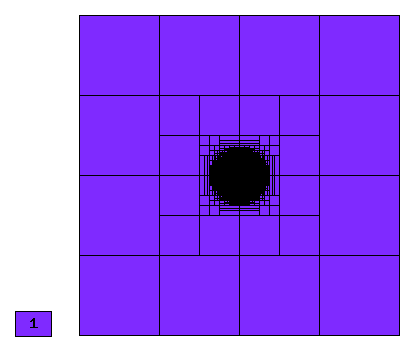
\includegraphics[height=5cm]{nist/nist-4/mesh_h1_aniso.png}\ \
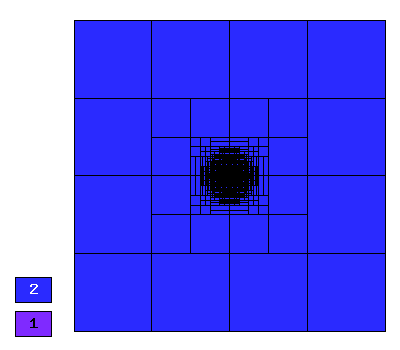
\includegraphics[height=5cm]{nist/nist-4/mesh_h2_aniso.png}
\caption{Final mesh for $h$-FEM anisotropic refinements with linear and quadratic elements.}
\label{fig:nist-4-h-aniso}
\end{figure}

Finally, Figs. \ref{fig:nist-4-conv} compare all
three approaches to automatic adaptivity from the point
of view of DOF and CPU convergence.

\begin{figure}[!ht]
\centering
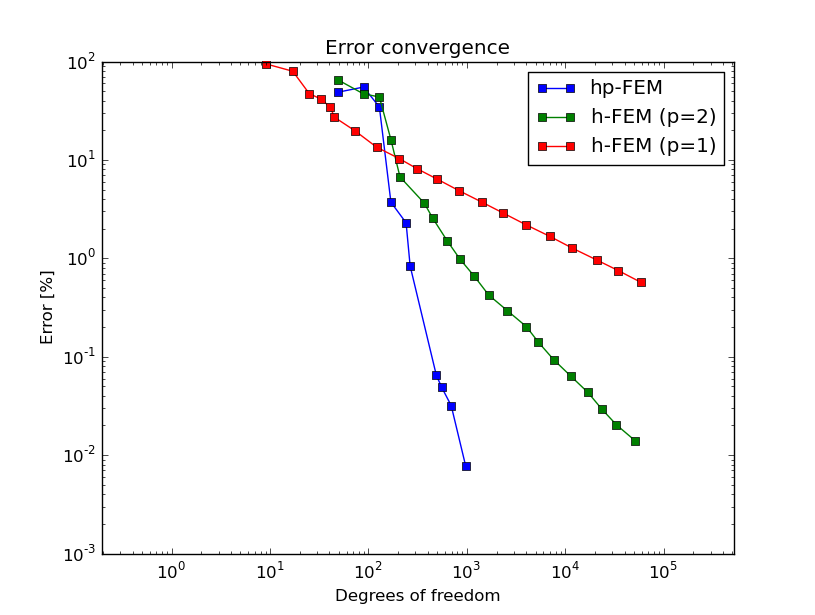
\includegraphics[height=5cm]{nist/nist-4/conv_dof_aniso.png}\ \
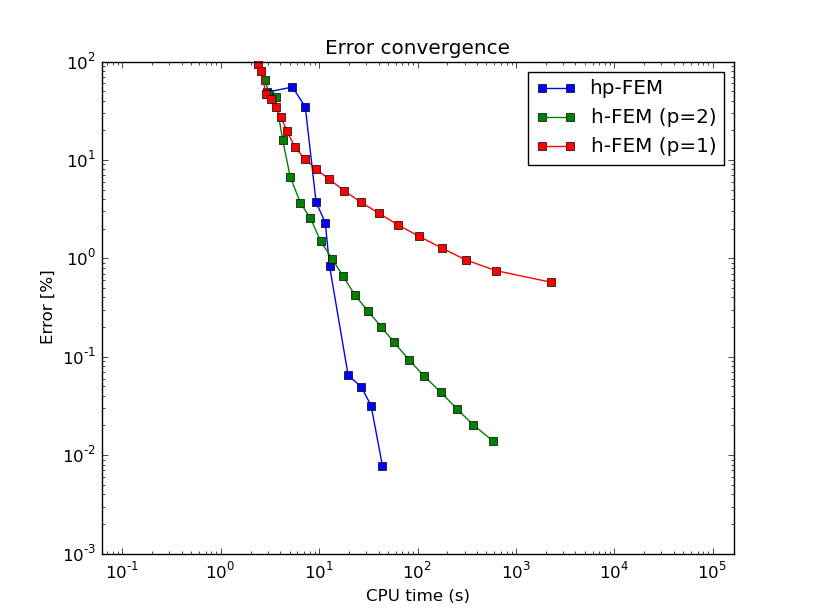
\includegraphics[height=5cm]{nist/nist-4/conv_cpu_aniso.png}
\caption{DOF and CPU time convergence graphs.}
\label{fig:nist-4-conv}
\end{figure}

